\documentclass[../../layout.tex]{subfiles}

\begin{document}
\chapter{Fundamentação teórica}
\hspace*{3em}O estudo, entendimento e compreensão dos conceitos abordados nesse projeto são de suma extema importância para sua compreensão.
do projeto.

\section{Internet das Coisas}
\hspace*{3em}\blindtext[1]
\subsection{Evolução da Internet das Coisas}
\hspace*{3em}\blindtext[1]
\subsection{Internet das Coisas e Indústria 4.0}
\hspace*{3em}\blindtext[1]

\section{Moddelo ultilizado para aplicação}
\hspace*{3em}Para o desenvolvimento da aplicação  utilizamos o modelo cliente servidor em três camadas, esse modelo permite a modularização da aplicação  em três camadas,  camada de interface com usuário, também conhecida como front end, camada lógica onde está inserida as regras de negócio também conhecido como backend e a camada de dados  onde realiza-se a comunicação com o banco de dados, essa arquitetura permite um desacoplamento de código que viabiliza a atualização das partes de forma independente e da tecnologia \cite{3layers}

\section{REST API}
\hspace*{3em}REST (Transferência representacional de estado) API (Interface de programação de aplicação) analisando os conceitos isolados.\par
API é um interface de comunicação  disponível por software com regras estabelecidas para que haja o entendimento de ambas as partes, esse conceito vem para criar uma camada de abstração, no qual para utilizar os recursos de um determinado software é apenas necessário o entendimento da interface  disponibilizada por um software eliminado a  necessidade do entendimento total do software, além de viabilizar o conceito de modularização  de arquitetura de software.\par \cite{16}
REST é um modelo de arquitetura criado para suprir conceitos de qualidade e funcionalidade, em princípio para sistemas distribuído. Mas acabou sendo utilizada largamente em servidores WEB, a arquitetura define um conjunto de restrições para uma arquitetura estilo REST como, padrões uniformes para interfaces, sem conservação de estado e desacoplamento total do cliente e servidor, com isso permitindo a interoperabilidade entre sistemas, quando um servidor WEB segue essa restrição pode ser denominado de REST FULL.\par
Portando uma REST API é um interface que aplica os conceito REST para sua implementação\cite{19}. Quando o protocolo HTTP é utilizando o URI (Identificador de recursos uniformes) se torna uma representação dos dados e os métodos HTTP são utilizados para manipular esses dados, como o método GET para recuperar os dados, o POST para criar novos dados, PUT para atualizar os dados e DELETE para apagar os dados \cite{16}.

\section{Backend}

\subsection{Conceito de backend}
\hspace*{3em}Uma aplicação WEB em geral é dividida  em duas principais partes, a camada do front end que é responsável pela interação com o usuário de forma gráfica e o back end é responsável por entregar toda a lógica necessária para o front end, geralmente o back end é dividido em três partes, aplicação, banco de dados  e servidor, esse elementos são responsáveis por implementar a lógica do negócio \cite{16}.

\subsection{Linguagem Banckend}
\hspace*{3em}A linguagem mais utilizada para programar dispositivos IoT é a linguagem C por ser mais otimizada para essa finalidade, mas por ser uma linguagem de baixo nível, exige uma extensa dedicação de tempo e torna-se moroso para soluções mais complexas. E para contornar essas deficiências a linguagem Elixir pode ser uma ótima alternativa. Por ser uma linguagem de alto  nível que não compromete tanto a performance do sistema.\par
A linguagem Erlang/Elixir é uma linguagem funcional desenvolvida para atingir alta performance e confiabilidade. Foi desenvolvida para aplicações voltadas para telecomunicações que exigem, baixa tolerancia de falhas, distribuida e real-time (tempo de execução). Por isso conta com um conjunto bibliotecas para desenvolvimento de sistemas de alta confiabilidade conhecida como OTP.\par
Elixir foi desenvolvida para ser executada na VM (máquina virtual) do Erlang nomeada como BEAM. A linguagem Elixir é relativamente nova mas já existem diversas aplicações que a utilizam e inclusive existem recursos para dispositivo embarcado como o framework Nerves \cite{ElixirorIoT} e para implementação de aplicações WEB como o framework Phoenix.

\subsection{Nerves}
\hspace*{3em}Nerves é um framework para desenvolvimento de projetos embarcados, baseado em Linux que apenas executa a VM BEAM, portanto proporcionando a utilização da linguagem Elixir para o desenvolvimento das aplicações, dessa forma desfrutando do potencial da linguagem para implementação de projetos embarcados. Além disso este framework proporciona diversas vantagens  em relação ao processo tradicional de programação de embarcados como, permite a fácil portabilidade para diferentes HW (hardware) embarcados e com uma vasta abrangência para diferentes HW embarcados, fácil manutenção e atualização de firmware por viabilizar a atualizações via OTA (atualização sobre o ar), dispensando o processo tradicional de dispor do acesso físico a flash do dispositivo para o armazenamento do firmware, proporciona também recursos para facilitar e agilizar o desenvolvimento de firmware e uma vasta biblioteca para manipulação dos sistemas embarcados\cite{nerves}.

\subsection{Phoenix}
\hspace*{3em}Phoenix é um framework desenvolvido em Elixir para implementação de aplicações WEB, que usa todo o potencial da linguagem Elixir, com isso desfrutando da concorrência fornecida pela VM BEAM, baixa tolerância a falha e baixa latência.  Além de aumentar o desempenho do desenvolvimento de  uma aplicação WEB também conta com diversos recurso que são disponibilizados de forma modular\cite{phoenix}.


\section{Frontend}
\hspace*{3em}\blindtext[1]

\begin{figure}[H]
\centering
\caption{Diagrama do software}
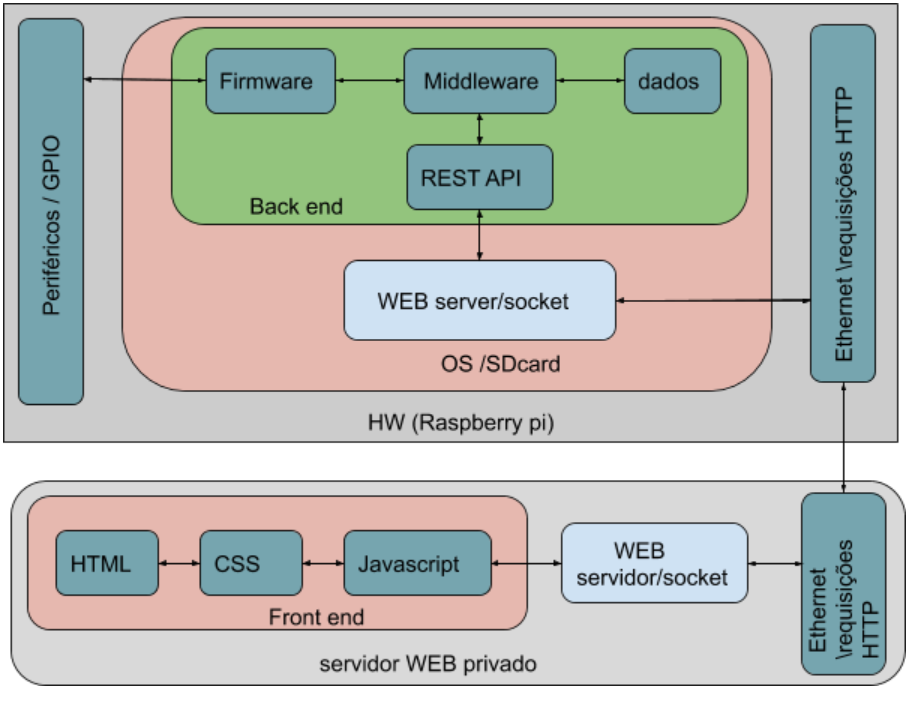
\includegraphics[width=0.5\textwidth]{assets/static/img/diagrama_tcc.PNG}
\label{fig:diagrama_sw}
\end{figure}

\section{Protocolos de comunicação} 
\hspace*{3em}\blindtext[1]
\subsection{i2c}
\hspace*{3em}\blindtext[1]
\subsection{1-wire}
\hspace*{3em}\blindtext[1]
\subsection{UART}
\hspace*{3em}\blindtext[1]

\section{Modelagem do Hardware}
\hspace*{3em}\blindtext[1]

\section{Sensores}
\hspace*{3em}\blindtext[1]

\section{Estrutura do Software}
\hspace*{3em}\blindtext[1]

\section{Método}
\hspace*{3em}\blindtext[1]

\end{document}
